\todo[inline, color=pink, size=normalsize]{Descrição geral do problema}

O uso de Veículos Aéreos Não Tripulados - do inglês \textit{Unmanned Aerial Vehicles} - UAVs - nos setores civil e militar têm crescido no últimos anos, uma vez que aeronaves desse tipo vêm sendo utilizadas na realização de missões de vigilância, reconhecimento e inspeção. Algumas das vantagens dos UAVs em relação às aeronaves tripuladas são a redução dos custos operacionais e dos riscos associados à presença de uma tripulação \cite{toledo_de_azevedo_pseudospectral_2018}. 

Missões de voo são comumente especificadas a partir da determinação de pontos que devem ser sequencialmente percorridos pela aeronave, os chamados \textit{waypoints}. Considerando-se que não existam obstáculos entre os \textit{waypoints} e que forças externas não atuem sobre a aeronave, o caminho mais rápido entre dois \textit{waypoints} é uma linha reta. No entanto, caso a aeronave esteja sujeita a um campo de vento, a determinação da trajetória se torna um problema de otimização complexo \cite{toledo_de_azevedo_pseudospectral_2018}. 

Nesta dissertação pretende-se determinar a trajetória a ser percorrida por um UAV para que o mesmo vá de um \textit{waypoint} inicial até um \textit{waypoint} final, consumindo a menor quantidade de bateria possível, enquanto atua sobre ele um campo de vento conhecido \cite{toledo_de_azevedo_pseudospectral_2018}. As variáveis empregadas na formulação das equações de movimento do UAV são representadas na Figura \ref{fig:uav:variaveis}:

\noindent	
\begin{minipage}{\textwidth}
	\vspace{\onelineskip}
	\centering
	\includegraphics[scale=0.25]{draw/resultados/pdf/uav}
	\captionof{figure}[Variáveis empregadas na formulação do problema  da otimização da trajetória de um UAV]{Variáveis empregadas na formulação das equações de movimento do UAV.}
	\label{fig:uav:variaveis}
	\vspace{\onelineskip}
\end{minipage}
%

Nesta figura, o UVA é modelado como um ponto com massa $ m $, com posição $ \big(d_x(t), d_y(t), d_z(t)\big) $ e velocidade $ \big(v_x(t), v_y(t), v_z(t)\big) $. O veículo se encontra submetido a ventos de velocidade $ \mathbf{c}(t) = \begin{bmatrix} c_x(t) & c_y(t) & c_z(t) \end{bmatrix} $ enquanto é impulsionado por uma força $ F(t) $. Os ângulos de atitude e de proa (\textit{heading}) são denotados, respectivamente, por $ \phi(t) $ e $ \theta(t) $. Por fim, $ c_d $ é o coeficiente de arrasto do ar e $ g $ a aceleração da gravidade. Tanto os \textit{waypoints} inicial ($ P_0 $) e final ($ P_f $), quanto o campo de vento ao qual está submetido o UAV são apresentados na Figura \ref{fig:uav:trajetoria}. 

\noindent	
\begin{minipage}{\textwidth}
	\vspace{\onelineskip}
	\centering
	\includegraphics[scale=0.45]{draw/resultados/pdf/uavTraj}
	\captionof{figure}[Campo de vento ao qual o UAV está submetido no problema  da otimização da trajetória]{Campo de vento ao qual o UAV está submetido no problema  da otimização da trajetória.}
	\label{fig:uav:trajetoria}
	\vspace{\onelineskip}
\end{minipage}

Neste estudo de caso assume-se que o UAV se mantém a uma altitude constante, logo, considera-se que o campo de vento atua somente no plano $ xy $. Nesse caso, para que a trajetória obtida seja devidamente avaliada, é interessante definir, para cada ponto da trajetória, se o campo de vento é favorável ou desfavorável ao movimento do UAV \cite{muppirala_finding_2020, teja_muppirala_finding_2013}. Para tanto, considera-se que o vento com velocidade $ c $ atua em um determinado ponto $ P(x,y) $, conforme ilustrado na Figura \ref{fig:uav:direcaoVento}. 

\noindent	
\begin{minipage}{\textwidth}
	\vspace{\onelineskip}
	\centering
	\includegraphics[scale=0.45]{draw/resultados/pdf/uavProjecaoVento}
	\captionof{figure}[Representação das variáveis utilizadas na definição da favorabilidade]{Representação das variáveis utilizadas na definição da favorabilidade $ f(x,y) $.}
	\label{fig:uav:direcaoVento}
	\vspace{\onelineskip}
\end{minipage}

Seja $ L $ a distância entre $ P(x,y) $ e $ P_f(r_x, r_y) $ e definida como: 
\begin{equation}
	\label{eq:uav:L}
	 L(x, y) = \sqrt{(y - r_y)^2 + (r_x - x)^2}
\end{equation} 
%
têm-se que:
%
\begin{subequations}
\begin{equation}
\sin(\beta) = \frac{y - r_y}{L} 
\end{equation}
\vspace{-0.5cm}
\begin{equation}
\cos(\beta) = \frac{x - r_x}{L} 
\end{equation}
\end{subequations}

Como $\alpha + \beta = \pi/2 $ rad, implica que $\cos(\alpha) = \sin( \beta )$. Portanto, as projeções de $ c_x(x,y) $ e $ c_y(x,y) $ na direção $ \overline{P  P_f} $ podem ser determinadas da seguinte forma:
%
\begin{subequations}
\begin{equation}
\label{eq:uav:cProjecoes}
c_h(x,y) = c_y(x,y) \cos(\alpha) = c_y(x,y) \sin(\beta) 
\end{equation}
\vspace{-0.7cm}
\begin{equation}
c_t(x,y) = c_x(x,y) \cos(\beta) 
\end{equation}
\end{subequations}

Neste caso, define-se $ f(x, y) $ como sendo a favorabilidade do campo de vento no ponto $ P(x, y) $, dada por  $ f(x, y) = c_t(x,y) - c_h(x,y) = c_x(x,y) \cos(\beta) - c_y(x,y) \sin(\beta)$. De posse destas informações é possível reescrever $ f(x,y) $ da seguinte maneira:
%
\begin{equation}
	f(x,y) = \frac{\big( r_x - x \big) c_x(x,y) + \big( r_y - y \big) c_y(x,y)}{\sqrt{(r_x - x)^2 + (r_y - y)^2 }}
\end{equation}  

O campo de vento é gerado atribuindo-se $ c_x(x, y) $ e $ c_y(x, y) $ aleatórios a pontos igualmente espaçados em $ x $ e $ y $. Desta forma, duas grades (matrizes) com 21 linhas e 11 colunas devem ser geradas, cada uma associada a uma componente de $ \mathbf{c}(x,y) $. As velocidades associadas aos pontos fora das grades são obtidas por meio de uma interpolação linear bidimensional. As matrizes contendo os valores de $ c_x(x, y) $ e $ c_y(x, y) $ empregadas na obtenção dos resultados aqui apresentados podem ser consultadas em \url{https://bitbucket.org/iasbeck/copilots/src/master/examples/uav/wind/loadWindX.m} e \url{https://bitbucket.org/iasbeck/copilots/src/master/examples/uav/wind/loadWindY.m}.

Na Figura \ref{fig:uav:campoVento} são representadas as velocidades e as favorabilidades associadas ao campo de vento em cada ponto $ (x,y) $. As zonas na cor verde são aquelas em que $ f(x,y) > 0 $ e nas quais o vento sopra na direção do \textit{waypoint} final $ P_f(r_x, r_y) $. Em contrapartida, as zonas representadas pela cor vermelha devem ser evitadas pelo UAV, isto é; são aquelas em que $ f(x,y) < 0 $ e o vento sobra para longe de $ P_f(r_x, r_y) $. As zonas na cor branca são aquelas em que $ f(x,y) \approx 0 $. As setas no gráfico representam os vetores de velocidade do vento $ \big( c_x(x,y), \, c_y(x,y) \big) $. Vale ressaltar que $ f(x,y) $ é dado em m/s, já que é definido como a soma das projeções das velocidades $ c_x(x,y) $ e $ c_y(x,y) $. 

\noindent	
\begin{minipage}{\textwidth}
	\vspace{\onelineskip}
	\centering
	\includegraphics[scale=0.5]{fig/resultados/uav/obs/wind}
	\captionof{figure}[Velocidades e favorabilidades associadas ao campo de vento para o problema da otimização da trajetória de um UAV]{Velocidades e favorabilidades associadas ao campo de vento para o problema da otimização da trajetória de um UAV.}
	\label{fig:uav:campoVento}
	\vspace{\onelineskip}
\end{minipage} 

\todo[inline, color=pink, size=normalsize]{Apresentação das equações dinâmicas - Equações, Estados, Controles e Valor inicial dos estados}

A dinâmica do UAV no plano $ xy $ é descrita como segue \cite{toledo_de_azevedo_pseudospectral_2018}: 
%
\begin{subequations}
\begin{equation}
\label{eq:uav:dinamica}
\dot{d}_x(t) = v_x(t),\;\;d_x(0) = r_{0x}\; \text{m}
\end{equation}
\vspace{-0.8cm}
\begin{equation}
\dot{d}_y(t) = v_x(t),\;\;d_y(0) = r_{0y}\; \text{m}
\end{equation}
\vspace{-0.8cm}
\begin{equation}
\dot{v}_x(t) = g \tan(\phi(t)) \cos(\theta(t)) - \frac{c_d}{m} \Big[ v_x(t) - c_x \big( d_x(t), d_y(t) \big) \Big],\;\; \\
			v_x(0) = 0 \; \text{m/s}
\end{equation}
\vspace{-0.8cm}
\begin{equation}
\dot{v}_y(t) = g \tan(\phi(t)) \sin(\theta(t)) - \frac{c_d}{m} \Big[ v_y(t) - c_y \big( d_x(t), d_y(t) \big) \Big],\;\;v_x(0) = 0 \; \text{m/s}
\end{equation}
\end{subequations}
%
em que $t$ é o tempo, $ \mathbf{x}(t) = \begin{bmatrix} d_x(t) & d_y(t) & v_x(t) & v_y(t) \end{bmatrix}^T $ é o vetor de variáveis de estado e $ \mathbf{u}(t) = \begin{bmatrix} \phi(t) & \theta(t) \end{bmatrix}^T $ é o vetor de variáveis de controle.

\todo[inline, color=pink, size=normalsize]{Apresentação da função objetivo}

Uma vez que deseja-se minimizar o consumo de bateria, propõe-se a minimização de $ J = \int_{0}^{t_f} I(t)dt$, sendo $ t_f $ o tempo final e $ I(t) $ a corrente que circula pelos terminais da bateria. Considerando-se que $ I(t) $ seja proporcional a $ F(t) $, de forma que $ I(t) = K_i \, F(t)$, e levando-se em conta que $ m \, g = F(t) \cos(\phi(t))$ para que a altitude do UAV se mantenha constante, é possível reescrever $ J $ da seguinte forma:
%
\begin{equation}
\label{eq:uav:J}
J = K_i \, m \, g \int_{0}^{t_f} \frac{1}{cos \, \phi(t)} dt
\end{equation}

\todo[inline, color=pink, size=normalsize]{Apresentação das restrições - Restrições laterais}

As restrições associadas à posição do UAV e aos controles $ \phi(t) $ e $ \theta(t) $ são definidas como seguem:
%
\begin{subequations}
\begin{equation}
\label{eq:uav:restricoesLaterais}
0 \leq d_x(t) \leq D_x
\end{equation}
\vspace{-0.7cm}
\begin{equation}
0 \leq d_y(t) \leq D_y
\end{equation}
\vspace{-0.7cm}
\begin{equation}
0 \leq \phi(t) \leq \Phi
\end{equation}
\vspace{-0.7cm}
\begin{equation}
-\pi \leq \theta(t) \leq \pi 
\end{equation}
\end{subequations}

\todo[inline, color=pink, size=normalsize]{Apresentação das restrições - Restrições terminais}

Ao fim da trajetória, o UAV deve estar posicionado a, no máximo, $ r $ m do \textit{waypoint} $ P_f(r_x, r_y) $. Tal condição é representada pela restrição terminal dada a seguir:
%
\begin{equation}
\label{eq:uav:restricaoTerminal}
\big( d_x(t_f) - r_x \big)^2 + \big( d_y(t_f) - r_y \big)^2 \leq r^2
\end{equation}

\todo[inline, color=pink, size=normalsize]{Apresentação das restrições - Restrições de caminho}

\todo[inline, color=pink, size=normalsize]{Tabela das constantes do problema}

A seguir estão listados os parâmetros utilizados neste estudo de caso \cite{toledo_de_azevedo_pseudospectral_2018}: massa do UAV ($ m = 0,5$ m), aceleração da gravidade ($ g = 0,81 $ m), coeficiente de arrasto do ar ($ c_d = 0,2 $ Ns/m), coordenada $ x $ do \textit{waypoint} final ($ r_x = 15 $ m), coordenada $ y $ do \textit{waypoint} final ($ r_y = 5 $ m), coordenada $ x $ do \textit{waypoint} inicial ($ r_{0x} = 1 $ m), coordenada $ y $ do \textit{waypoint} inicial ($ r_{0y} = 5 $ m), coeficiente de relação entre a força $ F(t) $ e a corrente elétrica $ I(t) $ ($ K_i = 5,08 $ A/N), limite superior para a posição do UAV na direção $ x $ ($ D_x = 20 $ m), limite superior para a posição do UAV na direção $ y $ ($ D_y = 10 $ m), limite superior para o ângulo de atitude ($ \Phi = \pi/6$ rad) e  máxima distância entre a posição final do UAV e o \textit{waypoint} final ($ r = 1 $ m).

\todo[inline, color=pink, size=normalsize]{Considerações específicas de cada problema - Inicialização do problema com duas execuções}

Cada resultado que será apresentado a seguir foi obtido a partir de duas execuções, sendo as informações sobre o campo de vento desconsiderados na primeira delas. Nesse caso, a solução obtida é uma linha reta que conecta os \textit{waypoints} $ P_0 $ e $ P_f $. Então, na segunda execução, o campo de vento é reinserido nas equações de movimento do UAV e a solução obtida na primeira execução é utilizada para a inicialização dos estados e controles. O tempo de processamento $ t_p $ e o número de avaliações da função objetivo $ n_{aval} $ requeridos por cada pacote foram computados a partir da soma dos $ t_p $ e $ n_{aval} $ em cada uma das duas execuções. Sem esta estratégia,  não é possível resolver o estudo de caso em análise via $ PSOPT $. Além disso, verifica-se que é possível, utilizando o $ COPILOTS $, determinar uma trajetória factível para o UAV sem que qualquer estimativa inicial. No entanto, obtém-se nesse caso $ t_p $ e $ n_{aval} $ mais elevados do que aqueles atribuídos às soluções obtidas via abordagem de inicialização aqui proposta. Empregando o $ FALCON $ é possível obter soluções, consideravelmente satisfatórias, sem que o usuário tenha que fornecer estimativas iniciais. Assim sendo, com o intuito de minimizar os $ t_p $ e $ n_{aval} $ atribuídos ao $ FALCON $, optou-se por deixar a inicialização dos estados e controles a cargo desse pacote e solucionar o estudo de caso em análise empregando-se uma única execução. 

\todo[inline, color=pink, size=normalsize]{Apresentação da análise de sensibilidade $ J \times N $ para definição de $ N_m $ }

São apresentados na Figura \ref{fig:uav:sensibilidade:J} os resultados referentes a influência do número de nós de colocação no melhor valor da função objetivo encontrada, bem como está identificada nestas figuras o número mínimo de nós de colocação $ N_m $. Para essa finalidade foram considerados trinta valores igualmente espaçados 5 e 179. \textcolor{red}{Para este estudo de caso, melhor solução é XXX. refeência}

\noindent	
\begin{minipage}{\textwidth}
	\vspace{\onelineskip}
	\centering
	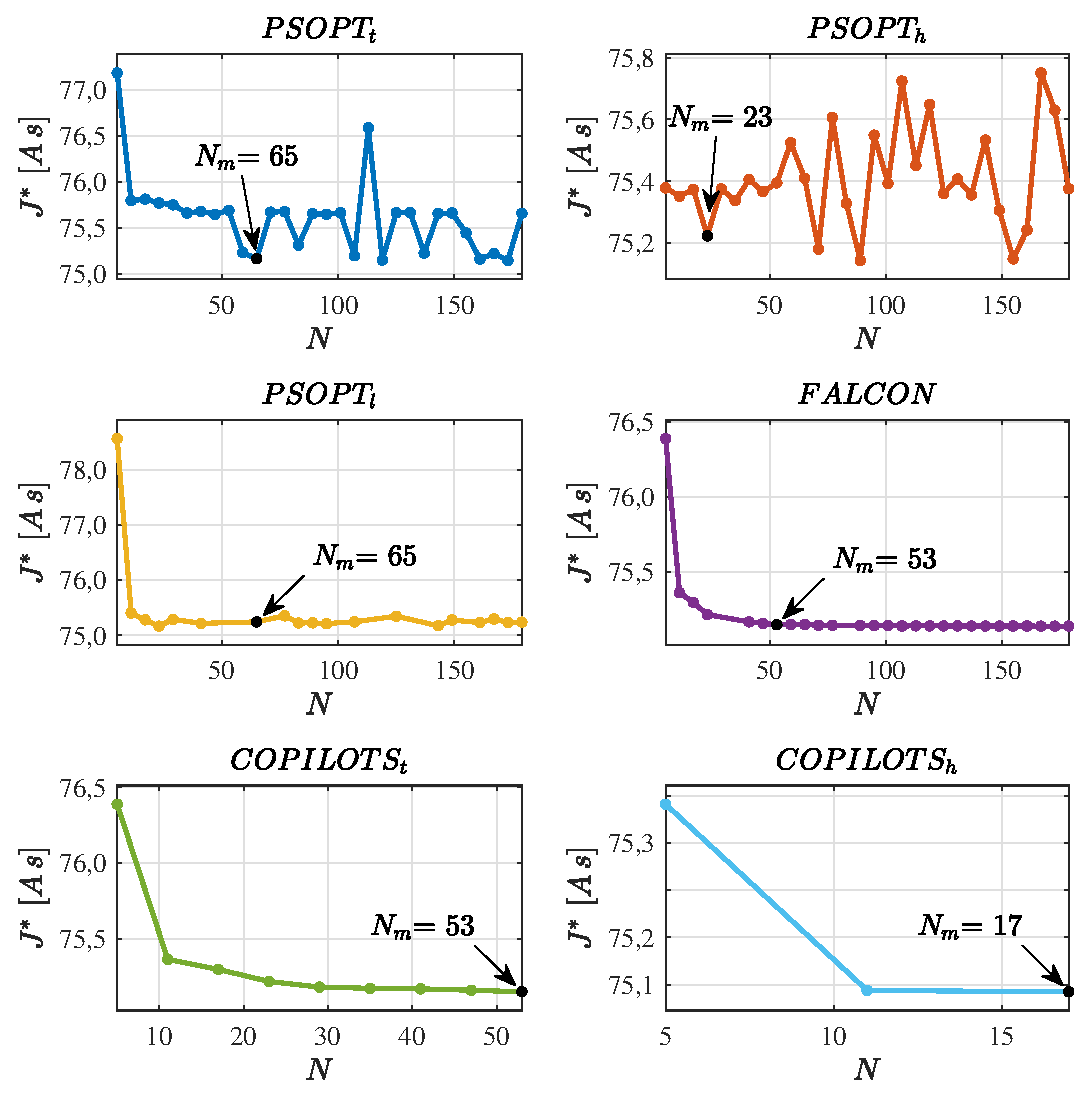
\includegraphics[scale=0.7]{fig/resultados/uav/sens/J}
	\captionof{figure}[Verificação da relação entre o número de nós de colocação e o valor ótimo da função objetivo para o problema do UAV]{Verificação da relação entre o número de nós de colocação $ N $ e o valor ótimo da função objetivo $ J^* $.}
	\label{fig:uav:sensibilidade:J}
	\vspace{\onelineskip}
\end{minipage}

\todo[inline, color=pink, size=normalsize]{Análise da análise de sensibilidade $ J \times N $}

Nesta figura observa-se que os valores de $ J^* $ referentes ao $ COPILOTS_t $ e ao $ COPILOTS_h $ não chegaram a convergir, uma vez que foram obtidas apenas 9 soluções empregando-se o primeiro, e 3 utilizando-se o segundo.  O valor de $ J^* $ obtido pelo $ PSOPT_h $ divergiu com o aumento de $ N $, uma vez que, no caso da colocação Hermite-Simpson, é necessário fornecer estimativas iniciais não só para os valores assumidos pelos estados e controles nos nós de colocação, mas também para aqueles assumidos pelos controles nos nós intermediários, o que dificulta a inicialização do PPNL. Já para o $ PSOPT_t $, este não divergiu com o aumento de $ N $, porém oscila em torno de um patamar para $ N > 65 $. Em contrapartida, o valor de $ J^* $ computado pelo $ PSOPT_l $ converge rapidamente, apresentando apenas leves oscilações à medida que $ N $ cresce. De fato, oscilações podem ser verificadas em todos os resultados atribuídos ao $ PSOPT $. Esse comportamento, provavelmente, está relacionado ao otimizador considerado neste pacote.  Vale ressaltar que os valores de $ J^* $ obtidos pelo $ FALCON $ convergiram suavemente, e sem que fossem verificadas quaisquer oscilações. Uma vez que não é possível verificar a convergência dos valores de  $ J^* $ para o $ COPILOTS_t $ e para o $ COPILOTS_h$, assume-se $ N_m = max\{N\} $.  No caso do $ PSOPT_t $, atribui-se a $ N_m $ o menor $ N $ em que se verifica um valor de $ J^* $ próximo a $ min\{J^*\} $. Por fim, considerando-se as bruscas variações observadas no $ PSOPT_h $, deve-se escolher $ N_m $ de forma subjetiva, buscando associar a essa métrica o menor $ N $ possível. 

Considerando os critérios de convergência originalmente adotados para a determinação de $ N_m $, deveria ser atribuído $ N_m = 23 $ ao $ PSOPT_l $. No entanto, a trajetória de $ \theta(t) $ obtida quando $ N = 23 $ (ver a Figura \ref{fig:uav:outsider23}), apresenta em $ t = 2,63 $ s um ponto consideravelmente distante dos demais, o que provavelmente se deve a alguma adversidade numérica no processo de otimização. Uma vez que a trajetória obtida via colocação pseudo-espectral é construída globalmente, utilizando-se somente um polinômio, distorções em um único nó de colocação podem fazer com que trajetórias consideravelmente oscilatórios sejam produzidas, como é o caso. Assim sendo, deve-se aumentar $ N_m $ até que o comportamento oscilatório seja eliminado. Na Figura \ref{fig:uav:outsider41} é apresentada a trajetória de $ \theta(t) $ obtida para $ N = 41 $, na qual verifica-se a redução das oscilações observadas inicialmente. Com base nesse novo critério, atribui-se ao $ PSOPT_l $ $ N_m = 65 $.

\noindent	
\begin{minipage}{\textwidth}
	\vspace{\onelineskip}
	\centering
	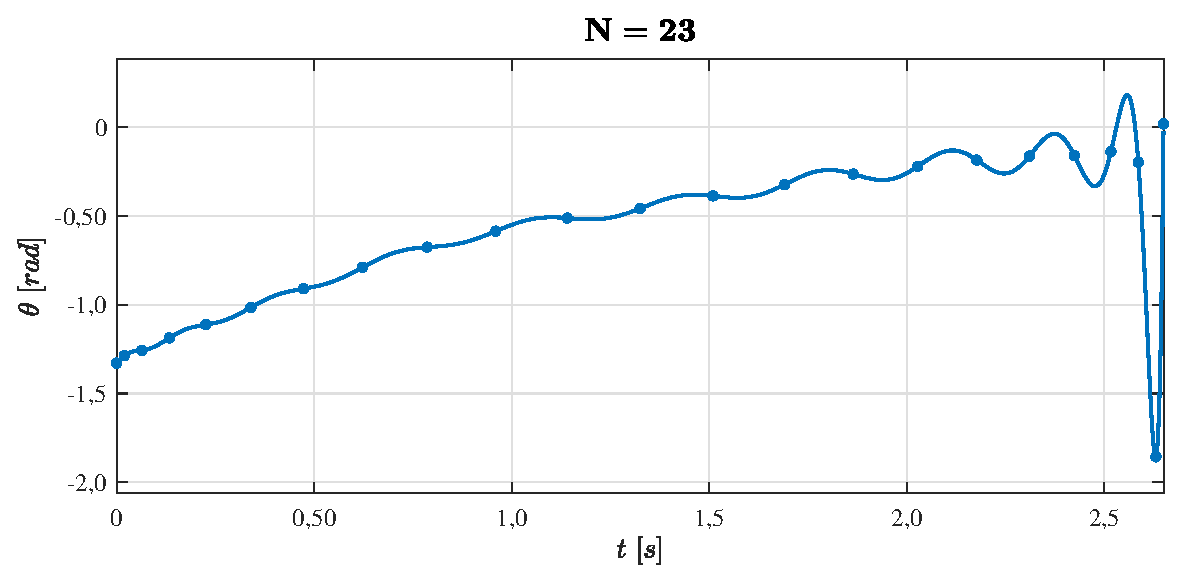
\includegraphics[scale=0.67]{fig/resultados/uav/obs/outsider23}
	\captionof{figure}[Trajetória do ângulo associado à projeção da força de sustentação no eixo $xy$ obtida utilizando-se 23 nós de colocação]{Trajetória de $ \theta(t) $ obtida para $ N = 23 $.}
	\label{fig:uav:outsider23}
	\vspace{\onelineskip}
\end{minipage}

Vale ressaltar que oscilações na trajetória de $ \theta(t) $ semelhantes às retratadas nas Figuras \ref{fig:uav:outsider23} e \ref{fig:uav:outsider41} foram reportadas por \citeonline{toledo_de_azevedo_pseudospectral_2018}. Tais oscilações ocorrem porque, ao fim da trajetória, $ \phi(t) $ aproxima-se de zero, o que faz com que a projeção horizontal de $ F(t) $ seja drasticamente reduzida. Assim sendo, quanto menor for $ \phi(t) $, menor será a influência de $ \theta(t) $ na trajetória do UAV. As oscilações atribuídas à trajetória de $ \theta(t) $ reportada em \citeonline{toledo_de_azevedo_pseudospectral_2018} são quase imperceptíveis, já que nesse caso adotou-se $ N = 80 $.

A  Tabela \ref{tab:uav:raw} apresenta um resumo das métricas obtidas por cada pacote. Neste destacam-se o valor da função objetivo ($ J^* $), o tempo de processamento médio ($ t_p $), o desvio padrão atribuído ($ s_t $), a máxima violação das restrições ($ \Delta c_{max} $) e o número de execuções bem sucedidas ($ N_s $).

\noindent	
\begin{minipage}{\textwidth}
	\vspace{\onelineskip}
	\centering
	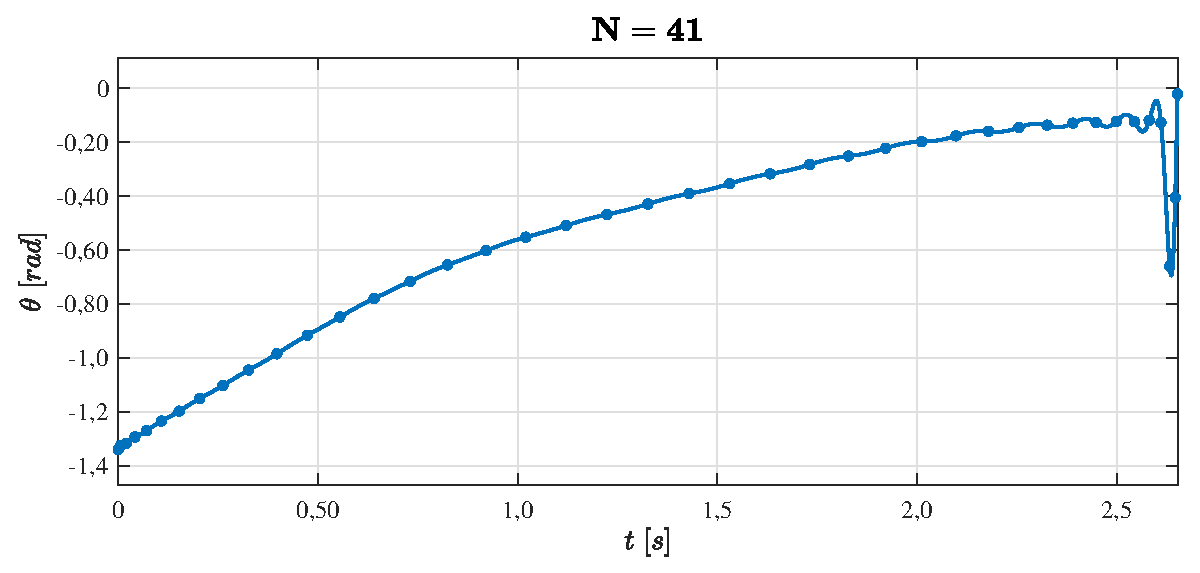
\includegraphics[scale=0.68]{fig/resultados/uav/obs/outsider41}
	\captionof{figure}[Trajetória do ângulo associado à projeção da força de sustentação no eixo $xy$ obtida utilizando-se 41 nós de colocação]{Trajetória de $ \theta(t) $ obtida para $ N = 41 $.}
	\label{fig:uav:outsider41}
	\vspace{\onelineskip}
\end{minipage}
 
\todo[inline, color=pink, size=normalsize]{Apresentação da tabela dos dados obtidos para $ N = N_m $}

\begin{table}[!h]
	\centering
	\caption[Métricas  obtidas  para  o  problema da otimização da trajetória de um UAV]{Métricas  obtidas  para  o  problema da otimização da trajetória de um UAV. Os melhores valores assumidos pelas métricas $ N_m $, $ J^* $, $ t_p $, $ n_{aval} $ e $ N_s\% $ estão em destaque.}
	\label{tab:uav:raw}
	\begin{tabular}{@{}ccccccccc@{}}
		\toprule
		Método       & $N_m$                              & $J^*$                                    & $t_p$ {[}$s${]}                         & $s_t$ {[}$s${]} & $n_{aval}$                          & $\Delta c_{max}$                         & $N_s$ & $N_s\%$                                  \\ \midrule
		$PSOPT_t$    & 65                                 & 75,16400                                 & 2,20747                                 & 0,23441         & {\color[HTML]{009901} \textbf{167}} & 6,97e-08                                 & 30    & {\color[HTML]{009901} \textbf{100,00\%}} \\
		$PSOPT_h$    & 23                                 & 75,22300                                 & {\color[HTML]{009901} \textbf{1,16775}} & 0,03329         & 360                                 & 7,63e-07                                 & 30    & {\color[HTML]{009901} \textbf{100,00\%}} \\
		$PSOPT_l$    & 65                                 & 75,24280                                 & 15,66657                                & 0,25870         & 800                                 & 4,08e-07                                 & 19    & 63,33\%                                  \\
		$FALCON$     & 53                                 & 75,14907                                 & 1,76303                                 & 0,03821         & 357                                 & 1,94e-10                                 & 27    & 90,00\%                                  \\
		$COPILOTS_t$ & 53                                 & 75,14907                                 & 587,37797                               & 0,71652         & 30821                               & 9,00e-09                                 & 9     & 30,00\%                                  \\
		$COPILOTS_h$ & {\color[HTML]{009901} \textbf{17}} & {\color[HTML]{009901} \textbf{75,14254}} & 238,48976                               & 0,58730         & 11860                               & 1,52e-10 & 3     & 10,00\%                                  \\ \bottomrule
	\end{tabular}
\end{table}

\todo[inline, color=pink, size=normalsize]{Análise dos dados obtidos para $ N = N_m $}

Nesta tabela nota-se que os valores de $ N_m $ associados aos métodos baseados na colocação trapezoidal são maiores que aqueles atribuídos aos que fazem uso da colocação Hermite-Simpson. Já o valor de $ N_m $ encontrado pelo $ PSOPT_l $ ficou tão grande quanto o atribuído ao $ PSOPT_t $. Isto se deve à adversidade numérica discutida anteriormente e representada nas Figuras \ref{fig:uav:outsider23} e \ref{fig:uav:outsider41}. Já o  $ COPILOTS_h $ foi o que obteve os menores de $ N_m $ e de $ J^* $, respectivamente, enquenato ao $ COPOLITS_t $ e ao $ COPILOTS_h $ estão relacionados os maiores valores de $ t_p $ e de $ n_{aval} $. 

Diferentemente do que foi observado nos resultados da maior parte dos outros estudos de caso já analisados nesta dissertação, não associam-se ao $ FALCON $ os menores valores de $ t_p $ e de $ n_{aval} $, apesar das métricas associadas a esse pacote terem encontrado valores bastante satisfatórios. Uma vez que a dinâmica associada ao estudo de caso depende da interpolação linear dos dados de uma tabela, o que atribui descontinuidades ao estudo de caso em análise \cite{betts_practical_2001}, não é possível que o $ FALCON $ compute as derivadas analíticas da dinâmica do UAV, pelo menos não daquela associada aos estados $ p_x(t) $ e $ p_y(t) $, o que prejudica o desempenho desse pacote. Os baixos valores de $ t_p $ e de $ n_{aval} $ relacionados ao $ FALCON $, apesar das descontinuidades, se devem ao fato desse pacote ter sido capaz de resolver o estudo de caso  empregando apenas uma execução, sem que fosse necessário uma estimativa inicial para os estados e controles. Ainda assim, somente considerando o $ FALCON $, o $ PSOPT_t $ e o $ PSOPT_h $, foi possível obter $ N_s\% $ satisfatórios (maiores que 90\%). 
 
O valor de $ t_p $ associado ao $ PSOPT_t $ é maior que aquele atribuído ao $ PSOPT_h $, provavelmente por que o $ N_m $ empregado pelo primeiro é consideravelmente maior que aquele utilizado pelo segundo. No entanto, o maior valor de $ n_{aval} $ foi obtido pelo $ PSOPT_h $. Por fim, vale ressaltar que os valores de $ t_p $ e de $ n_{aval} $ referentes ao $ PSOPT_l $ são bem maiores que os associados ao $ PSOPT_t $ e ao $ PSOPT_h $, mesmo que os $ N_m $ relacionados ao $ PSOPT_l $ e ao $ PSOPT_t $ sejam iguais. 

\todo[inline, color=pink, size=normalsize]{Apresentação das trajetórias de estados e controles}

As trajetórias referentes as variáveis de estado e controle considerando-se $ N = N_m $ são apresentadas nas Figuras \ref{fig:uav:x:d_x} à \ref{fig:uav:u:theta}.

\noindent
\begin{minipage}{\textwidth}
	\vspace{\onelineskip}
	\centering
	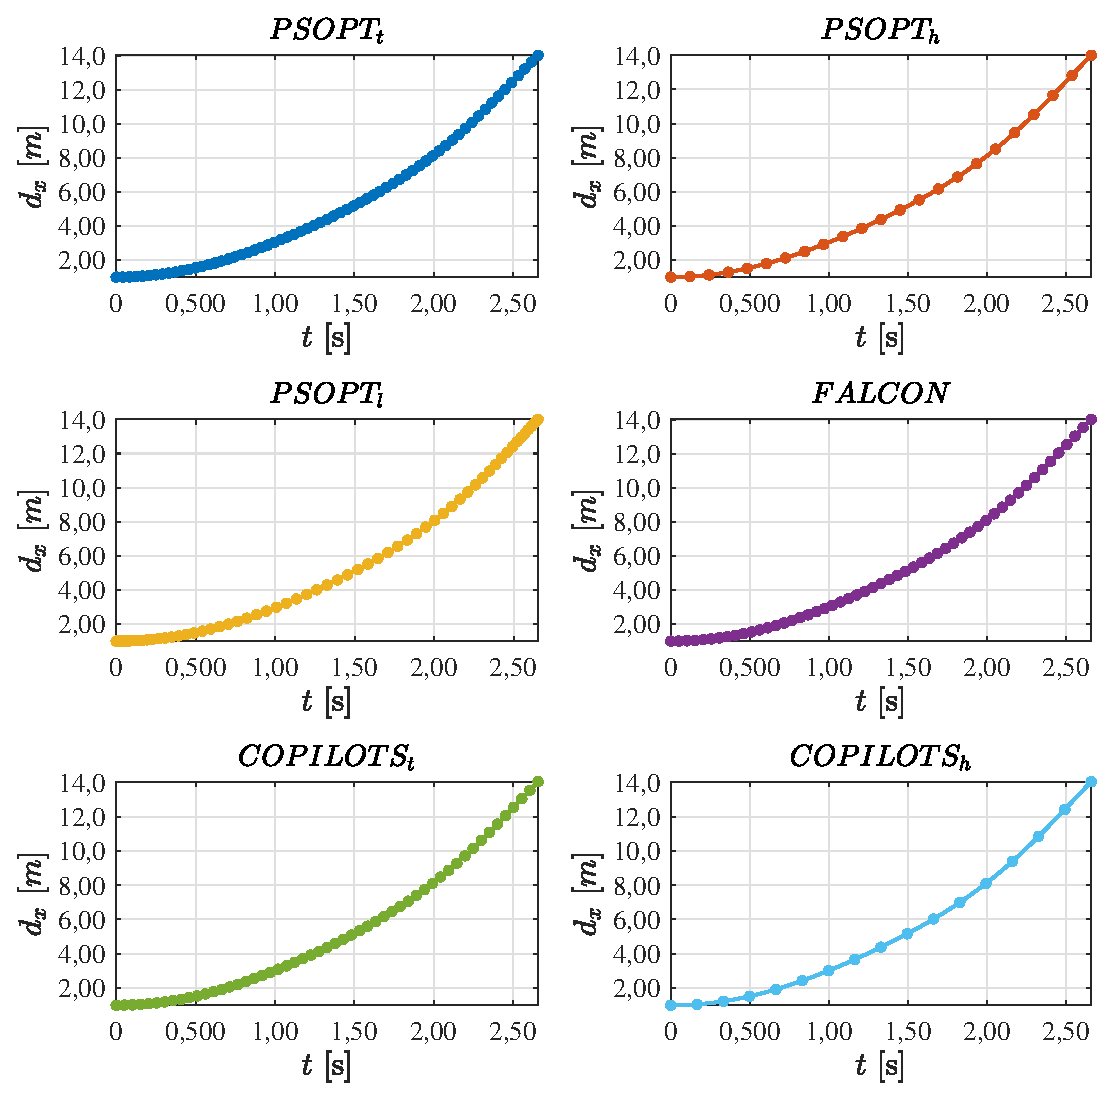
\includegraphics[scale=0.7]{fig/resultados/uav/traj/x/d_x}
	\captionof{figure}[Trajetórias da posição do UAV no eixo $x$]{Trajetórias do estado $ d_x(t) $ obtidas por meio do emprego de cada um dos métodos em análise. Os pontos representam os valores assumidos por $ d_x(t) $ nos nós de colocação, enquanto as linhas contínuas representam as trajetórias interpoladas a partir desses pontos.}
	\label{fig:uav:x:d_x}
	\vspace{\onelineskip}
\end{minipage}

\noindent
\begin{minipage}{\textwidth}
	\vspace{\onelineskip}
	\centering
	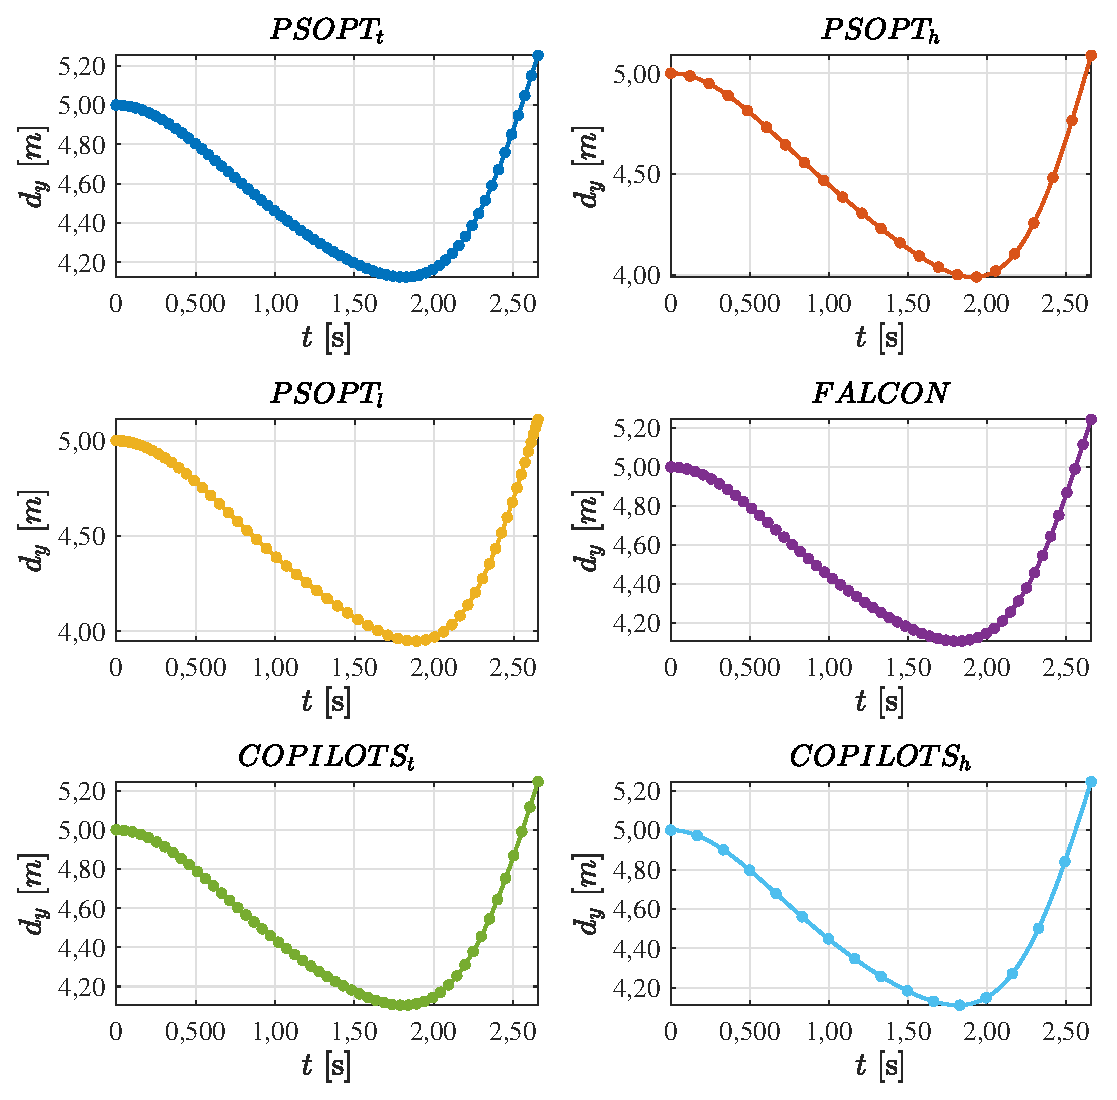
\includegraphics[scale=0.7]{fig/resultados/uav/traj/x/d_y}
	\captionof{figure}[Trajetórias da posição do UAV no eixo $y$]{Trajetórias do estado $ d_y(t) $ obtidas por meio do emprego de cada um dos métodos em análise. Os pontos representam os valores assumidos por $ d_y(t) $ nos nós de colocação, enquanto as linhas contínuas representam as trajetórias interpoladas a partir desses pontos.}
	\label{fig:uav:x:d_y}
	\vspace{\onelineskip}
\end{minipage}

\noindent
\begin{minipage}{\textwidth}
	\vspace{\onelineskip}
	\centering
	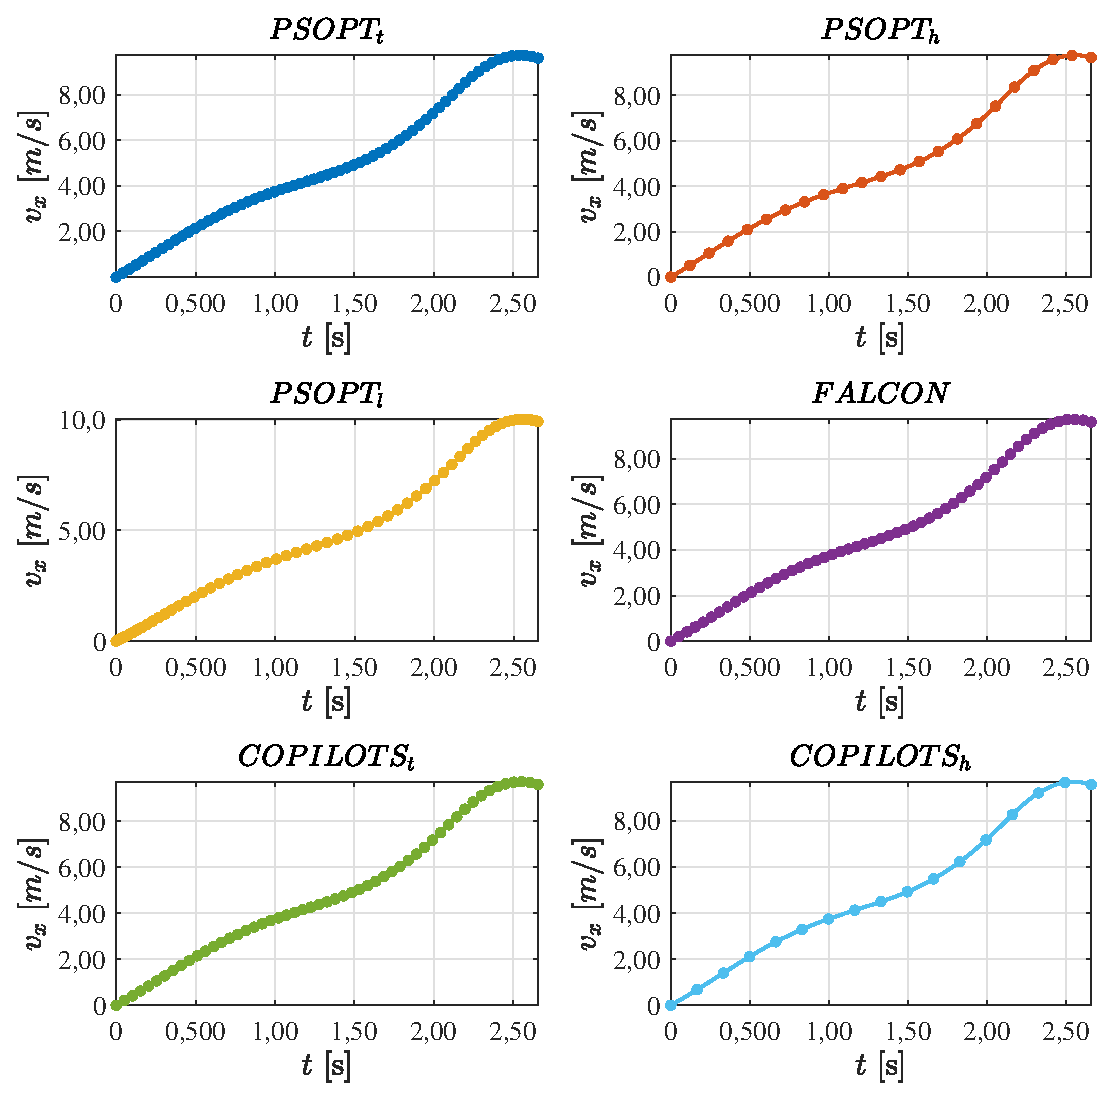
\includegraphics[scale=0.7]{fig/resultados/uav/traj/x/v_x}
	\captionof{figure}[Trajetórias da velocidade do UAV no eixo $x$]{Trajetórias do estado $ v_x(t) $ obtidas por meio do emprego de cada um dos métodos em análise. Os pontos representam os valores assumidos por $ v_x(t) $ nos nós de colocação, enquanto as linhas contínuas representam as trajetórias interpoladas a partir desses pontos.}
	\label{fig:uav:x:v_x}
	\vspace{\onelineskip}
\end{minipage}

\noindent
\begin{minipage}{\textwidth}
	\vspace{\onelineskip}
	\centering
	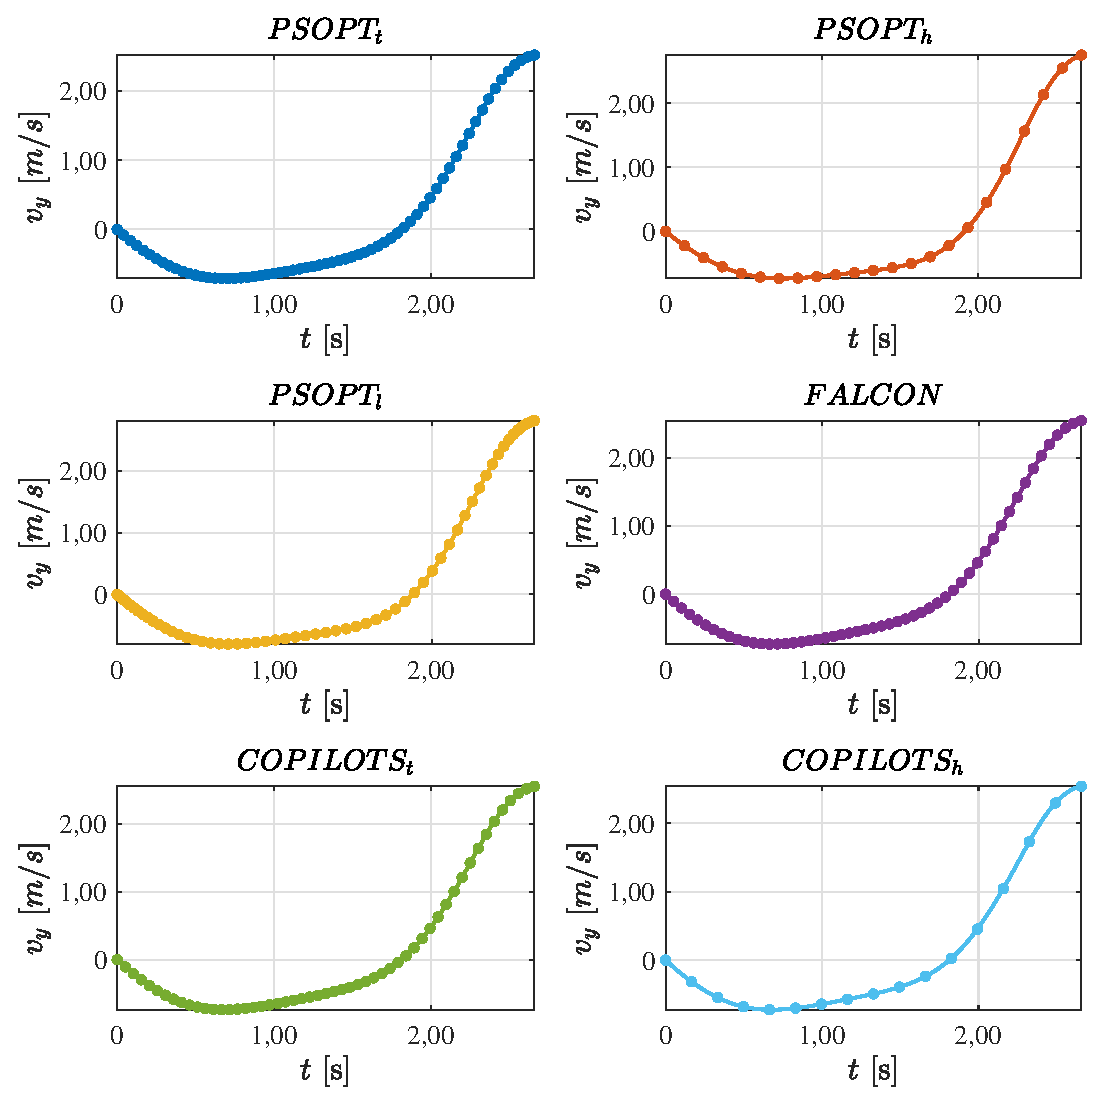
\includegraphics[scale=0.7]{fig/resultados/uav/traj/x/v_y}
	\captionof{figure}[Trajetórias da posição do UAV no eixo $y$]{Trajetórias do estado $ v_y(t) $ obtidas por meio do emprego de cada um dos métodos em análise. Os pontos representam os valores assumidos por $ v_y(t) $ nos nós de colocação, enquanto as linhas contínuas representam as trajetórias interpoladas a partir desses pontos.}
	\label{fig:uav:x:v_y}
	\vspace{\onelineskip}
\end{minipage}

\noindent
\begin{minipage}{\textwidth}
	\vspace{\onelineskip}
	\centering
	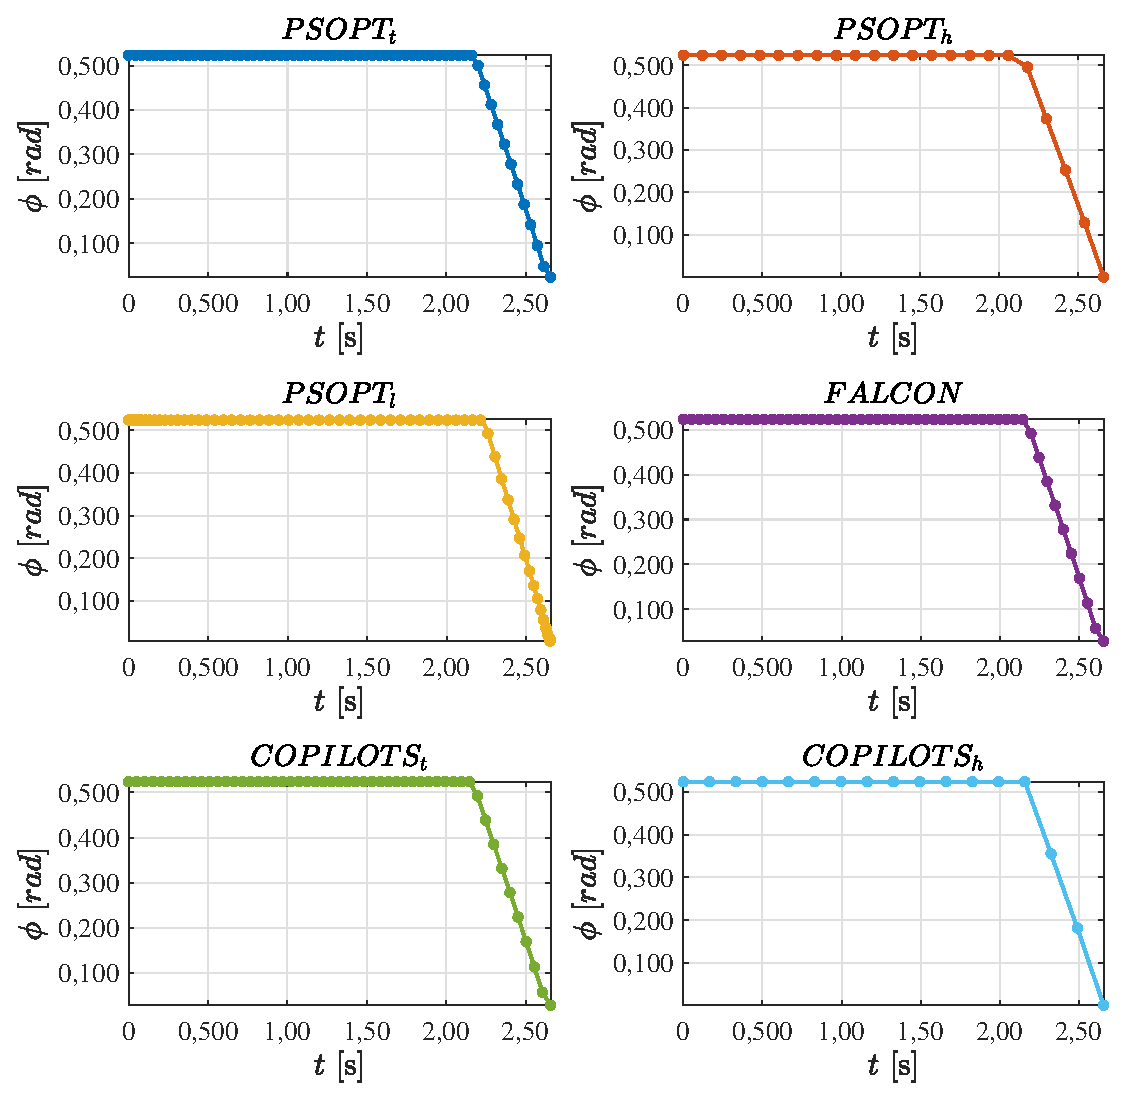
\includegraphics[scale=0.7]{fig/resultados/uav/traj/u/phi}
	\captionof{figure}[Trajetórias do ângulo entre a força de sustentação e a vertical]{Trajetórias do controle $ \phi(t) $ obtidas por meio do emprego de cada um dos métodos em análise. Os pontos representam os valores assumidos por $ \phi(t) $ nos nós de colocação, enquanto as linhas contínuas representam as trajetórias interpoladas a partir desses pontos.}
	\label{fig:uav:u:phi}
	\vspace{\onelineskip}
\end{minipage}

\noindent
\begin{minipage}{\textwidth}
	\vspace{\onelineskip}
	\centering
	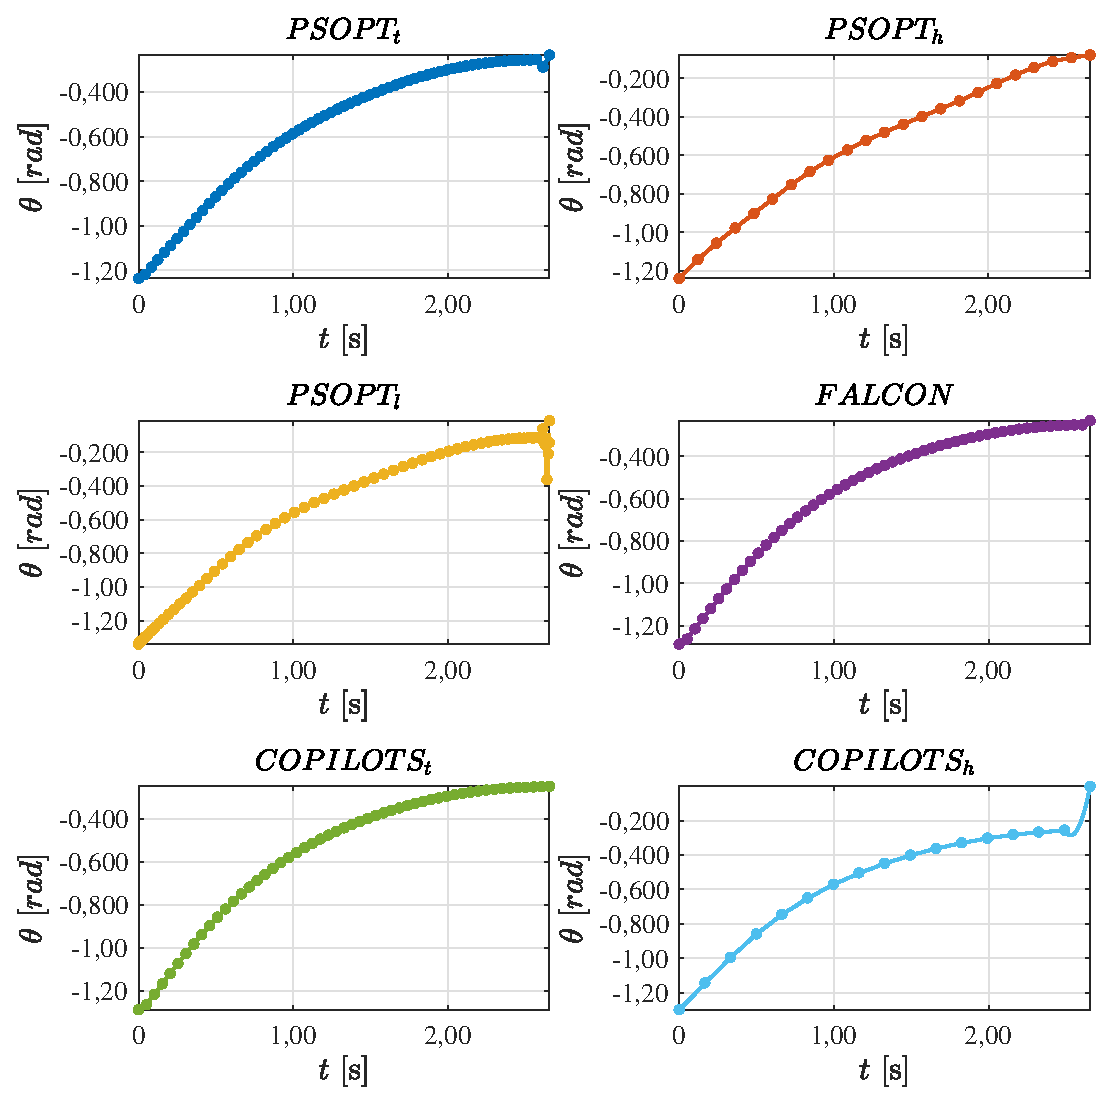
\includegraphics[scale=0.7]{fig/resultados/uav/traj/u/theta}
	\captionof{figure}[Trajetórias do ângulo associado à projeção da força de sustentação no eixo $xy$]{Trajetórias do controle $ \theta(t) $ obtidas por meio do emprego de cada um dos métodos em análise. Os pontos representam os valores assumidos por $ \theta(t) $ nos nós de colocação, enquanto as linhas contínuas representam as trajetórias interpoladas a partir desses pontos.}
	\label{fig:uav:u:theta}
	\vspace{\onelineskip}
\end{minipage}

\todo[inline, color=pink, size=normalsize]{Análise das trajetórias de estados e controles}

De forma geral, pode-se observar que as trajetórias de $ d_x(t) $, $ d_y(t) $, $ v_x(t) $, e $ v_y(t) $ obtidas por meio de cada um dos métodos se mostraram muito semelhantes uma às outras. Verifica-se o mesmo com as trajetórias do controle $ \phi(t) $. As oscilações na trajetória do controle $ \theta(t) $ associada ao $ PSOPT_l $ já foram discutidas e se encontram representadas nas Figura \ref{fig:uav:outsider23} e \ref{fig:uav:outsider41}. No entanto, a partir da análise dos resultados ilustrados na Figura \ref{fig:uav:u:theta}, é possível verificar que tais oscilações aparecem também nas trajetórias associadas ao $ PSOPT_t $, ao $ FALCON $ e ao $ COPILOTS_h $. Mesmo que tenha sido atribuído a esse último pacote um baixo $ N_m $, é possível verificar que a trajetória associada ao mesmo não foi globalmente afetada pela presença de oscilações. Esse resultado se deve à forma como a trajetória é interpolada a partir dos nós de colocação quando empregada a colocação Hermite-Simpson. Nesse caso, vários polinômios distintos compõe a trajetória, sendo cada um deles responsável pelos valores atribuídos à mesma entre dois nós de colocação específicos. Conclui-se que, apesar de proporcionar a geração de trajetórias mais suaves, a interpolação global empregada no caso da colocação pseudo-espectral possui a desvantagem de ser globalmente afetada por perturbações em qualquer um dos nós de colocação. 

\todo[inline, color=pink, size=normalsize]{Apresentação dos gráficos de trajetória complexos caso haja}

Na Figura \ref{fig:uav:avancado} estão representados a vista superior da trajetória do UAV e o campo de vento que atua sob o mesmo. Este gráfico foi elaborado a partir dos resultados obtidos via $ COPILOTS_h $, pacote ao qual associa-se o menor $ J^* $. Os pontos destacados em azul no gráfico representam os valores assumidos por $ d_x(t) $ e $ d_y(t) $ nos nós de colocação, enquanto a linha continua que conecta esses pontos representa a trajetória computada com base nas trajetórias descritas nas Figuras \ref{fig:uav:x:d_x} e  \ref{fig:uav:x:d_y}. 

\noindent
\begin{minipage}{\textwidth}
	\vspace{\onelineskip}
	\centering
	\includegraphics[scale=0.55]{fig/resultados/uav/obs/adv}
	\captionof{figure}[Vista superior da trajetória do UAV e campo de vento que atua sob o mesmo]{Vista superior da trajetória do UAV e campo de vento que atua sob o mesmo.}
	\label{fig:uav:avancado}
	\vspace{\onelineskip}
\end{minipage}

\todo[inline, color=pink, size=normalsize]{Apresentação das análises de sensibilidade $ N \times t_p $ e $ N \times n_{aval} $}

A influência do número de nós de colocação no tempo de processamento e no número de avaliações da função objetivo são apresentadas nas Figuras \ref{fig:uav:sensibilidade:t} e \ref{fig:uav:sensibilidade:naval}. Nestes gráficos são apresentadas as variações: $ \Delta t_p = \max\{t_p\} - \min\{t_p\} $ e $ \Delta n_{aval} = \max\{n_{aval}\} - \min\{n_{aval}\} $. Os pontos nos gráficos representam os valores atribuídos a $ t_p $ (e a $ n_{aval} $) para cada um dos $ N $ considerados, enquanto as linhas contínuas representam curvas de tendência, obtidas por meio de regressões lineares, em que $R^2$ é o coeficiente de determinação. Os valores de $ N $ empregados na geração desses resultados são iguais àqueles considerados na computação da relação entre $ J^* $ e $ N $. 

\noindent
\begin{minipage}{\textwidth}
	\vspace{\onelineskip}
	\centering
	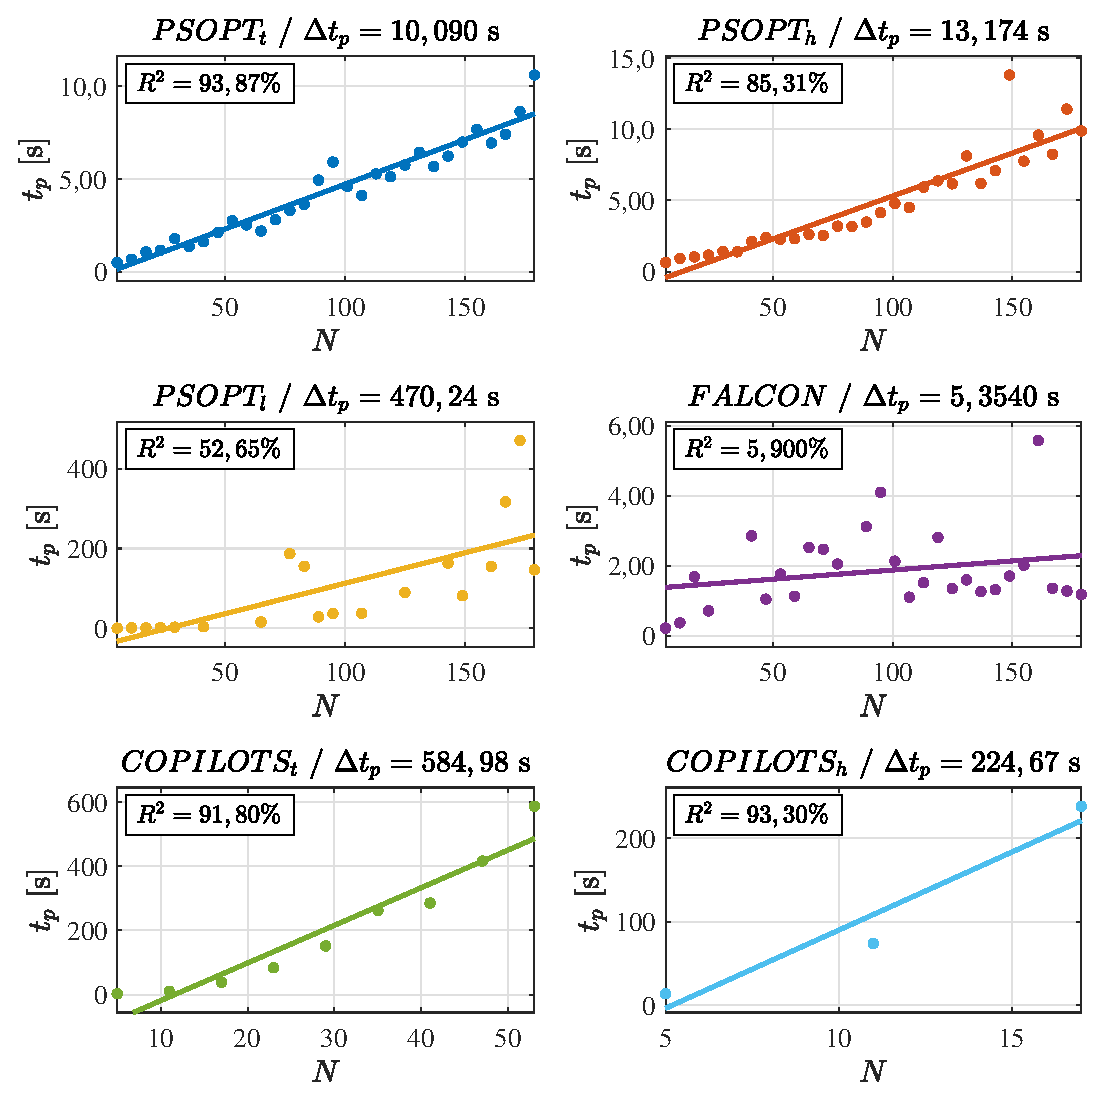
\includegraphics[scale=0.7]{fig/resultados/uav/sens/t}
	\captionof{figure}[Relação entre o tempo de processamento e o número de nós de colocação para o problema do UAV]{Relação entre o tempo de processamento $ t_p $ e o número de nós de colocação $ N $, considerando cada um dos métodos em análise.}
	\label{fig:uav:sensibilidade:t}
	\vspace{\onelineskip}
\end{minipage}

Nestes gráficos observa-se que há uma relação quase linear entre os $ N $ e $ t_p $ associados ao $ PSOPT_t $ e ao $ PSOPT_h $. No entanto, não é possível dizer o mesmo da relação entre os $ N $ e $ n_{aval} $ para os valores encontrados pelo $ PSOPT_l $. Já no caso do $ FALCON $ não foi possível verificar qualquer relação direta entre $ N $ e $ t_p $ ou entre $ N $ e $ n_{aval} $. Tais alegações podem ser verificadas a partir da análise dos respectivos valores de $ R^2 $. Vale ressaltar ainda que os coeficientes de determinação computados pelo $ COPILOTS_t $ e pelo $ COPILOTS_h $ não são representativos, uma vez que as regressões referentes a esses pacotes foram baseadas em um número muito pequeno de pontos. 

Os valores de $ t_p $ associados ao $ FALCON $ são consideravelmente menos sensíveis ao aumento de $ N $ que aqueles atribuídos ao $ PSOPT_t $, ao $ PSOPT_h $ e ao $ PSOPT_l $. De fato, o $ \Delta t_p $ associado ao $ FALCON $ é cerca de 90 vezes maior que o atribuído ao $ PSOPT_l $ por exemplo. No entanto, o $ n_{aval} $ associado ao $ FALCON $ é tão alto quanto àquele atribuído ao $ PSOPT_h $, mesmo que os resultados obtidos por meio do $ FALCON $ tenham sido determinados em uma única execução, e apesar dos métodos que empregam a colocação Hermite-Simpson normalmente estarem vinculados a $ n_{aval} $ maiores que aqueles que fazem uso da colocação trapezoidal. De fato, o valor de $ n_{aval} $ associado ao $ PSOPT_t $, por exemplo, é quase duas vezes menor que o atribuído ao $ PSOPT_h $. O fraco desempenho do $ FALCON $ pode ser justificado pela impossibilidade de determinarem-se as derivadas analíticas das equações de movimento do UAV, que dependem da interpolação linear dos dados. 

\noindent
\begin{minipage}{\textwidth}
	\vspace{\onelineskip}
	\centering
	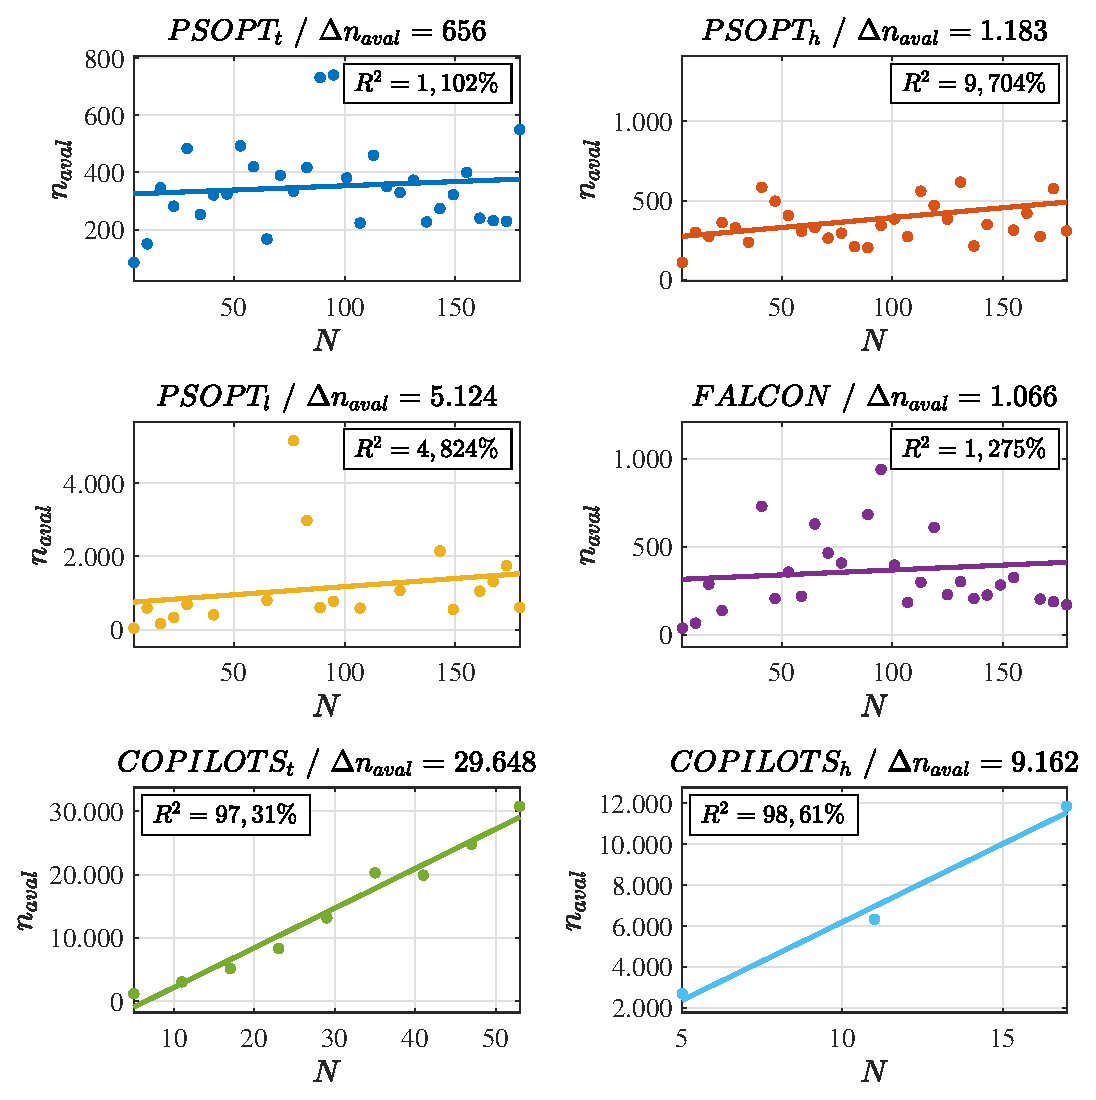
\includegraphics[scale=0.7]{fig/resultados/uav/sens/eval}
	\captionof{figure}[Relação entre o número de avaliações da função objetivo e o número de nós de colocação]{Relação entre o número de avaliações da função objetivo $ n_{aval} $ e o número de nós de colocação $ N $, considerando cada um dos métodos em análise.}
	\label{fig:uav:sensibilidade:naval}
	\vspace{\onelineskip}
\end{minipage}

\todo[inline, color=pink, size=normalsize]{Análise das análises de sensibilidade $ N \times t_p $ e $ N \times n_{aval} $}

Os valores de $ \Delta t_p $ e de $ \Delta n_{aval} $ referentes  ao $ PSOPT_l $ são consideravelmente maiores que aqueles atribuídos ao $ PSOPT_t $ e ao $ PSOPT_h $, o que indica que as métricas associadas a esse pacote são mais sensíveis ao aumento de $ N $. Já o valor de $ \Delta n_{aval} $ associado ao $ COPILOTS_t $ é muito maior do que aqueles reportados pelos demais métodos, mesmo que o máximo valor para $ N $ seja consideravelmente baixo (igual a 53). De forma análoga, o maior $ \Delta t_p $ encontra-se vinculado ao $ COPILOTS_t $. 

Por fim, vale ressaltar que não deve-se comparar os valores de $ \Delta n_{aval} $ e de $ \Delta t_p $ associados ao $ COPI - LOTS_h $ com aqueles atribuídos aos demais pacotes, uma vez que somente três soluções distintas foram obtidas por meio do $ COPILOTS_h $ e que o máximo $ N $ associado a esse pacote é igual a 17. Por exemplo, não seria correto concluir, apenas por meio da análise do valor de $ \Delta t_p $, que o $ n_{aval} $ associado ao $ COPILOTS_h $ é menos sensível ao aumento de $ N $ que aquele atribuído ao $ PSOPT_l $.

\todo[inline, color=pink, size=normalsize]{Observações adicionais sobre os resultados obtidos no estudo de caso - Instabilidade na geração da trajetória atribuída ao pseudo-espectral}
